%-------------------------------------------------------------------------------
%-------------------------------------------------------------------------------
%-------------------------------------------------------------------------------
\chapter{DS3 : Mines 2016
Graphe du WEB}
%-------------------------------------------------------------------------------
%-------------------------------------------------------------------------------
%-------------------------------------------------------------------------------
\section*{Préliminaire concernant la programmation}
%-------------------------------------------------------------------------------
%-------------------------------------------------------------------------------
%-------------------------------------------------------------------------------
Il faudra coder des fonctions à l'aide du langage de programmation OCaml, tout autre langage étant exclu. Lorsque le candidat écrira une fonction, il 
pourra faire appel à d'autres fonctions définies dans les questions précédentes ; il pourra aussi définir des fonctions auxiliaires. Quand l'énoncé 
demande de coder une fonction, il n'est pas nécessaire de justifier que celle-ci est correcte, sauf si l'énoncé le demande explicitement. Enfin, si les 
paramètres d'une fonction à coder sont supposés vérifier certaines hypothèses, il ne sera pas utile dans l'écriture de cette fonction de tester si les 
hypothèses sont bien vérifiées.

\medskip

Dans les énoncés, un même identificateur écrit dans deux polices de caractères différentes désignera la même entité, mais du point de vue mathématique pour la police en italique (par exemple $n$) et du point de vue informatique pour celle en romain avec espacement fixe (par exemple \type{n}).

%-------------------------------------------------------------------------------
%-------------------------------------------------------------------------------
%-------------------------------------------------------------------------------
\section{Présentation}
%-------------------------------------------------------------------------------
%-------------------------------------------------------------------------------
%-------------------------------------------------------------------------------
Le {\sf World Wide Web}, ou Web, est un ensemble de pages (identifiées de manière unique par leurs adresses, ou {\sf URL} pour {\sc Uniform Resource Locators}, de la forme

\type{http://mines-ponts.fr/index.php}) reliées les unes aux autres par des hyperliens. 
Le Web est souvent modélisé comme un graphe orienté dont les sommets sont les pages Web et les arcs les hyperliens entre pages. 
Le Web étant potentiellement infini, on s'intéresse à des sous-graphes du Web obtenus en naviguant sur le Web, c'est-à-dire en le parcourant page par page, en suivant les hyperliens d'une manière bien déterminée. Ce parcours du Web pour en collecter des sous-graphes est réalisé de manière automatique par des logiciels 
autonomes appelés Web crawlers ou crawlers en anglais, ou collecteurs en français.
%-------------------------------------------------------------------------------
%-------------------------------------------------------------------------------
\newpage
%-------------------------------------------------------------------------------
\section{Fonctions utilitaires}
%-------------------------------------------------------------------------------
%-------------------------------------------------------------------------------
%-------------------------------------------------------------------------------
Nous allons tout d'abord coder certaines fonctions de manipulation de structures de données de base, qui seront utiles dans le reste de l'exercice.
%-------------------------------------------------------------------------------
%-------------------------------------------------------------------------------
\begin{Exercise}\it
Écrire une fonction \type{renverse : 'a liste -> 'a list} qui renvoie la liste passée en paramètre retournée ; on n'utilisera pas \type{List.rev}. \type{renverse [4; 2; 3]} renvoie \type{[3; 2; 4]}.
\end{Exercise}
%-------------------------------------------------------------------------------
\begin{Answer}
La récursivité terminale produit un résultat souvent inversé.
\begin{lstlisting}
let renverse liste =
   let rec aux reste fait =
       match reste with
       |[] -> fait
       |t::q -> aux q (t :: fait)
    in aux liste [];;      
\end{lstlisting}
\end{Answer}
%-------------------------------------------------------------------------------
%-------------------------------------------------------------------------------
\begin{Exercise}\it
On part d'une liste \type{liste} de type \type{(a * a list) list}, c'est une liste de couples 

\type{[(x1, l1) ; ... ; (xn, ln)]}, où chaque \type{xi} (lire $x_i$) est un élément de type \type{'a}, et \type{li} (lire $l_{i}$) une liste d'éléments de type \type{'a} de la forme \type{[yi1 ; ... ;yipi]}.
\type{yij} se lit $y_{i, j}$ et \type{yipi}, $y_{i, p_i}$.

Coder une fonction \type{aplatir : (a * a list) list -> a list}, telle que \type{aplatir liste} est une liste d'éléments de type \type{'a} :
\begin{lstlisting}
[x1;y11;...;y1p1;x2;y21;...;y2p2;...;xn;yn1;...;ynpn]
\end{lstlisting}
\end{Exercise}
%-------------------------------------------------------------------------------
\begin{Answer}
\begin{lstlisting}
let rec aplatir liste =
   match liste with
   |[] -> []
   |(w,l)::reste -> (w::l) @ (aplatir reste);;      
\end{lstlisting}
\end{Answer}
%-------------------------------------------------------------------------------
%-------------------------------------------------------------------------------
\begin{Exercise}\it 
Coder une fonction \type{tri\_fusion : (a * b) list -> (a * b) list} triant une liste de couples $(x, y)$ par ordre décroissant de la valeur de la seconde composante $y$ de chaque couple. On devra utiliser l'algorithme de tri par fusion (aussi appelé \og  tri fusion \fg ). 

Donner, sans démonstration, la complexité de cet algorithme.
\end{Exercise}
%-------------------------------------------------------------------------------
\begin{Answer}
On commence par découper la liste en deux parties presque de même longueur.
\begin{lstlisting}
let rec decouper liste = 
   match liste with
   |x::y::q -> let (l1, l2)=decouper q in
               x::l1, y::l2
   |_ -> liste, [] ;;
\end{lstlisting}

On doit savoir fusionner deux listes triées
\begin{lstlisting}
let rec fusion l1 l2 = 
   match l1, l2 with
   |[], _ -> l2
   |_, [] -> l1
   |(a1, b1)::q1, (a2, b2)::q2 when b1 < b2 -> (a2, b2)::(fusion l1 q2)
   |t1::q1, t2::q2 -> t1::(fusion q1 l2);;
\end{lstlisting}
Il reste à tout combiner
\begin{lstlisting}
let rec tri_fusion liste = 
   match liste with
   |[] -> []
   |[t] -> [t]
   |_ -> let l1, l2 = decouper liste in
         fusion (tri_fusion l1) (tri_fusion l2);;
\end{lstlisting}
\end{Answer}
%-------------------------------------------------------------------------------
%-------------------------------------------------------------------------------
\subsection{Dictionnaires}
%-------------------------------------------------------------------------------
%-------------------------------------------------------------------------------
On va utiliser dans la suite du problème un type de données \type{dictionnaire} qui permet de stocker des couples formés d'une chaîne de caractères (une clef) et d'un entier (une valeur). On dit que le dictionnaire associe la valeur à la clef. A chaque clef présente dans le dictionnaire est associée une seule valeur. Les fonctions suivantes sont supposées être prédéfinies :
\begin{itemize}
\item \type{dictionnaire\_vide : unit -> dictionnaire}.\\
l'appel \type{dictionnaire\_vide ()} crée un nouveau dictionnaire vide.
\item \type{ajoute : string -> int -> dictionnaire -> dictionnaire}.\\
l'appel \type{ajoute clef valeur dict} renvoie un nouveau dictionnaire identique au dictionnaire \type{dict}, sauf qu'un couple \type{(clef, valeur)} y a été ajouté.
\item \type{contient : string -> dictionnaire -> bool}.\\
l'appel \type{contient clef dict} renvoie un booléen indiquant s'il y a un couple dont la clef est \type{clef} dans le dictionnaire \type{dict}. 
\item \type{valeur : string -> dictionnaire -> int}.\\
l'appel \type{valeur clef dict} renvoie la valeur associée à la clef \type{clef} dans le dictionnaire \type{dict}. Cette fonction ne peut être appelée que si la clef est présente dans le dictionnaire.
\end{itemize}
%-------------------------------------------------------------------------------
%-------------------------------------------------------------------------------
\begin{Exercise}\it 
Écrire les fonctions ci-dessus si on implémente le dictionnaire par des listes de couples :
\begin{lstlisting}
type dict = (string * int) list;;
\end{lstlisting}
Quelle la complexité des fonctions écrites en fonction du nombre $n$ d'entrées dans le dictionnaire ?
\end{Exercise}
%-------------------------------------------------------------------------------
\begin{Answer}
On commence par deux fonctions de complexité constante
\begin{lstlisting}
let dictionnaire_vide () = [];;

let ajoute cle k dico = (cle, k) :: dico;;
\end{lstlisting}

\newpage

Les deux suivantes, semblables, sont de complexité en ${\cal O}(n)$.
\begin{lstlisting}
let rec contient cle dico = 
   match dico with
   |[] -> false
   |(ch, k)::q when ch = cle -> true
   |_::q -> contient cle q;;

let rec valeur cle dico = 
   match dico with
   |[] -> failwith "Clé non présente"
   |(ch, k)::q when ch = cle -> k
   |_::q -> valeur cle q;;
\end{lstlisting}
\end{Answer}
%-------------------------------------------------------------------------------
%-------------------------------------------------------------------------------
Les chaînes de caractères sont comparables par les opérateurs classiques, \type{<, >, <=, >=}.

On peut implémenter aussi les dictionnaires par des arbres binaires :
\begin{lstlisting}
type arbre = Vide | Noeud of arbre * string * int * arbre;;

let dictionnaire_vide () = Vide;;
\end{lstlisting}
%-------------------------------------------------------------------------------
%-------------------------------------------------------------------------------
\begin{Exercise}\it 
Quelle propriété doivent vérifier les chaînes des nœuds de l'arbre pour obtenir des dictionnaires dont la complexité, que l'on donnera sans démonstration, est meilleure que dans la question précédente ?

On supposera que les arbres restent équilibrés.
\end{Exercise}
%-------------------------------------------------------------------------------
\begin{Answer}
On doit avoir une structure d'arbre binaire de recherche : pour tout nœud $n_0$, les chaînes des nœuds du fils gauche (resp. du fils droit) doivent être inférieures (resp.supérieures) à la chaîne de $n_0$.
La complexité est lors un ${\cal O}(h)$ où $h$ est la hauteur.

Dans le cas d'arbres équilibrés la hauteur est une ${\cal O}\bigl(\log(n)\bigr)$.
\end{Answer}
%-------------------------------------------------------------------------------
%-------------------------------------------------------------------------------
\begin{Exercise}\it 
Écrire la fonction \type{contient}.

Expliquer simplement comment modifier la fonction  \type{contient} en la fonction \type{valeur}.
\end{Exercise}
%-------------------------------------------------------------------------------
\begin{Answer}
\begin{lstlisting}
let rec contient cle dico =
   match dico with
   |Vide -> false
   |Noeud(g, ch, k, d) when ch = cle -> true
   |Noeud(g, ch, k, d) when ch > cle -> contient cle g
   |Noeud(g, ch, k, d) -> contient cle d;;   
\end{lstlisting}
Pour la fonction \type{valeur} on renvoie une erreur dans le premier cas, on renvoie $k$ dans le second et on remplace \type{contient} par \type{valeur} dans les appels récursifs des autres cas.
\end{Answer}
%-------------------------------------------------------------------------------
%-------------------------------------------------------------------------------
On supposera écrite la fonction \type{ajoute}.

\medskip

Dans toute la suite on supposera que les complexités des fonctions \type{ajoute}, \type{contient} et \type{valeur} est en ${\cal O}\bigl(\log(n)\bigr)$ où $n$ est le nombre d'entrées du dictionnaire. 
%-------------------------------------------------------------------------------
%-------------------------------------------------------------------------------
\begin{Exercise}\it
Coder \type{unique : string list -> string list * dictionnaire}, qui est telle que l'appel \type{unique liste} renvoie un couple \type{(liste', dict)} où \type{liste'} est la liste des chaînes de caractères de liste distinctes (dans l'ordre de leur première occurrence dans liste) et où \type{dict} associe à chaque chaîne de caractères dans \type{liste'} sa position dans \type{liste'} (en numérotant à partir de 0). \end{Exercise}
%-------------------------------------------------------------------------------
\begin{Answer} On utilise une fonction auxiliaire dont les paramètres sont la liste restant à traiter, la liste déjà construite, le dictionnaire déjà construit et l'indice du premier terme à ajouter
\begin{lstlisting}
let unique liste = 
   let rec aux reste fait dico k =
       match reste with
       |[] -> renverse fait, dico
       |cle::q when contient cle dico -> aux q fait dico k
       |cle::q -> aux q (cle::fait) (ajoute cle k dico) (k + 1) 
   in aux liste [] (dictionnaire_vide ()) 0;;
       
\end{lstlisting}
\end{Answer}
%-------------------------------------------------------------------------------
%-------------------------------------------------------------------------------

{\bf Exemple} : l'appel \type{unique ["x"; "zz"; "x"; "x"; "zz"; "yt"]} renvoie un couple formé de la liste \type{["x"; "zz"; "yt"]} et d'un dictionnaire associant à \type{"x"} la valeur \type{0}, à \type{"zz"} la valeur \type{1} et à \type{"yt"} la valeur \type{2}.
%-------------------------------------------------------------------------------
%-------------------------------------------------------------------------------
\begin{Exercise}\it
Quelle est la complexité de la fonction \type{unique} en terme de la longueur $n$ de la liste $liste$ en argument et du nombre $m$ d'éléments distincts dans la liste $liste$~? Justifier la réponse.
\end{Exercise}
%-------------------------------------------------------------------------------
\begin{Answer}

On peut majorer le coût des fonctions \type{contient} et \type{ajoute} par un ${\cal O}\bigl(\log(m)+1\bigr)$ car le dictionnaire contient au plus $m$ éléments ; on ajoute 1 car $m$ peut rester égal à 1.
Ainsi la complexité de \type{aux} est majorée par un ${\cal O}\bigl(n\log(m)+n\bigr)$ ; la fonction \type{renverse} n'ajoutant qu'un ${\cal O}(n)$.

\newpage
\end{Answer}
%-------------------------------------------------------------------------------
%-------------------------------------------------------------------------------
%-------------------------------------------------------------------------------
\section{Crawler simple}
%-------------------------------------------------------------------------------
%-------------------------------------------------------------------------------
%-------------------------------------------------------------------------------
Nous allons maintenant implémenter un crawler simple en OCaml. 

On suppose fournie une fonction \type{recupere\_liens : string -> string list} prenant en argument l'URL d'une page Web $p$ et renvoyant la liste des URL des pages $q$ pour lesquelles il existe un hyperlien de $p$ à $q$, dans l'ordre lexicographique.

Pour illustrer le comportement de cette fonction, nous considérons un exemple de mini-graphe du Web à six pages et neuf hyperliens comme suit :
\begin{center}
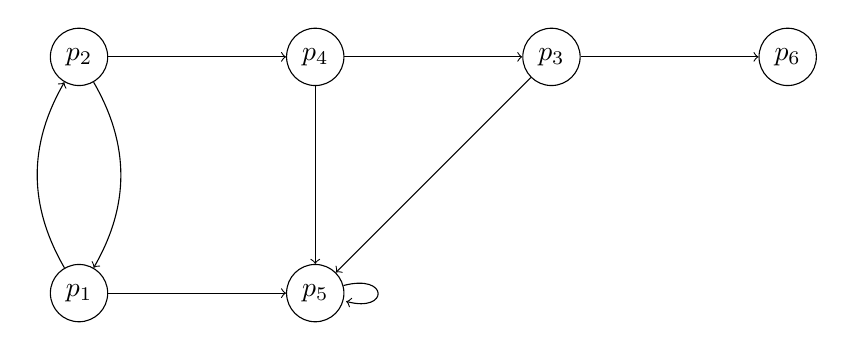
\begin{tikzpicture}[every node/.style={draw,circle}]
\node (A) at (0, 1) {$p_1$};
\node (B) at (0, 4) {$p_2$};
\node (C) at (3, 1) {$p_5$};
\node (D) at (3, 4) {$p_4$};
\node (E) at (6, 4) {$p_3$};
\node (F) at (9, 4) {$p_6$};
\draw[->] (A) edge[bend left] (B);
\draw[->] (A) -- (C);
\draw[->] (B) edge[bend left] (A);
\draw[->] (B) -- (D);
\draw[->] (D) -- (C);
\draw[->] (D) -- (E);
\draw[->] (E) -- (C);
\draw[->] (E) -- (F);
\draw[->] (C) edge [loop right] (C);
\end{tikzpicture}
\end{center}


Dans cette représentation, $p_1$, $p_2$, etc., sont les URL de pages Web (simplifiées pour l'exemple), et les arcs représentent les hyperliens entre pages Web.

Dans ce mini-graphe, un appel à \type{recupere\_liens "p1"} retourne la liste \type{["p2"; "p5"]}.

Un crawler est un programme qui, à partir d'une URL et d'un entier $n$, parcourt le graphe du Web en visitant progressivement les pages dont les liens sont présents dans chaque page rencontrée, en suivant une stratégie de parcours de graphe (par exemple, largeur d'abord, ou profondeur d'abord). À chaque nouvelle page, si celle-ci na pas déjà été visitée, tous ses hyperliens sont récupérés et ajoutés à une liste de liens à traiter. 

{\bf N.B.} {\sf Le sujet demande donc d'utiliser une liste pour implémenter une pile ou une file dans les parcours ci-dessous. On notera que, selon que l'on adjoint la liste des voisins (avec l'opérateur \lstinline{@}) d'un coté ou de l'autre, on construit une file ou une pile.}

Le processus s'arrête quand Le crawler a visité $n$ pages distinctes et donc appelé $n$ fois la fonction \type{recupere\_liens} (sauf s'il n'y a plus de pages à visiter).

Les fonctions \type{crawler} renvoient en sortie une liste de longueur au plus $n$ de couples \type{(v,  l)} où \type{v} est l'URL d'une page visitée (les pages apparaissant dans l'ordre où elles ont été visitées) et \type{l} la liste des liens récupérés sur la page \type{v}.
Ce résultat est appelé un {\it crawl}.

On utilisera une variable de type dictionnaire pour se souvenir des pages déjà visitées.
%-------------------------------------------------------------------------------
%-------------------------------------------------------------------------------
\begin{Exercise}\it 
Coder \type{crawler\_bfs : int -> string -> (string * string list) list} qui prend en entrée un nombre $n$ de pages et une URL \type{u} et renvoie un crawl. On demande que \type{crawler\_bfs} parcoure
le graphe du Web en suivant une stratégie en largeur d'abord (breadth-first search), c'est-à-dire en visitant en priorité les pages rencontrées le plus tôt dans l'exploration.  
\end{Exercise}
%-------------------------------------------------------------------------------
\begin{Answer}
\begin{lstlisting}
let crawler_bfs n page =
   let rec aux pages vus n liste = 
      match n, liste with
      |0, _ -> renverse pages
      |_, [] -> renverse pages
      |_, p::q when contient p vus -> aux pages vus n q
      |_, p::q -> let l = recupere_liens p in
                  aux ((p, l)::pages) (ajoute p 17 vus) (n-1) (q @ l)
   in aux [] (dictionnaire_vide ()) n [page];;
\end{lstlisting}
Les 4 paramètres de la fonction auxiliaire sont
\begin{enumerate}
    \item les pages déjà visitées, dans l'ordre inverse,
    \item le dictionnaire des pages vues, avec une valeur inutilisée,
    \item le nombre de pages restant à découvrir,
    \item la liste des pages en attente.
\end{enumerate}

Les deux premiers cas du pattern-matching correspondent à la fin de la recherche, soit on a vu assez de pages, soit il n'y ap lus de nouvelles pages à visiter.

Le troisième cas passe une page déjà visitée.

Le dernier cas traite une nouvelle page : on l'ajoute au dictionnaire et aux pages vues et on ajoute ses liens {\bf à droite} des pages à voir pour obtenir un parcours en largeur.

On notera qu'on n'a pas optimisé la fonction :
\begin{itemize}
    \item on ne teste pas si une page a déjà été visitée avant de l'ajouter dans la file
    \item l'ajout a une complexité linéaire à cause de la concaténation alors que la complexité peut être constante (en moyenne) dans un type bien écrit.
\end{itemize}
\end{Answer}
%-------------------------------------------------------------------------------
%-------------------------------------------------------------------------------
Par exemple, sur le mini-graphe, \type{crawler\_bfs 4 "p1"} pourra renvoyer le résultat :

\type{["p1", ["p2"; "p5"]; "p2", ["p1"; "p4"]; "p5", ["p5"]; "p4", ["p3"; "p5"]]}
%-------------------------------------------------------------------------------
%-------------------------------------------------------------------------------
\begin{Exercise}\it 
Coder \type{crawler\_bfs : int -> string -> (string * string list) list} qui prend en entrée un nombre $n$ de pages et une URL \type{u} et renvoie un crawl. On demande que\type{crawler\_dfs} parcoure le graphe du Web en suivant une stratégie en profondeur d'abord (depth-first search), c'est-à-dire en visitant en priorité les pages rencontrées le plus récemment dans l'exploration. 
\end{Exercise}
%-------------------------------------------------------------------------------
\begin{Answer}
On peut écrire une fonction analogue en adjoignant en tête
\begin{lstlisting}
let crawler_dfs n page =
   let rec aux pages vus n liste = 
      match n, liste with
      |0, _ -> renverse pages
      |_, [] -> renverse pages
      |_, p::q when contient p vus -> aux pages vus n q
      |_, p::q -> let l = recupere_liens p in
                  aux ((p, l)::pages) (ajoute p 17 vus) (n-1) (l @ q)
   in aux [] (dictionnaire_vide ()) n [page];;
\end{lstlisting}
\newpage
\end{Answer}
%-------------------------------------------------------------------------------
%-------------------------------------------------------------------------------
Par exemple, sur le mini-graphe, \type{crawler\_dfs 4 "p1"} pourra renvoyer le résultat :

\type{["p1", ["p2"; "p5"]; "p2", ["p1"; "p4"]; "p4", ["p3"; "p5"]; "p3", ["p5"; "p6"]]}
%-------------------------------------------------------------------------------
%-------------------------------------------------------------------------------
\begin{Exercise}\it 
Coder une fonction OCaml \type{construit\_graphe} de signature
\begin{lstlisting}
(string * string list) list -> string list * int vect vect
\end{lstlisting}
telle que si \type{crawl} est le résultat renvoyé par un crawler alors \type{construit\_graphe crawl} est un couple \type{(l, G)} où \type{l} est une liste de toutes les URL de pages contenues dans la liste \type{crawl} et \type{G} est la matrice d'adjacence du sous-graphe partiel du Web restreint aux pages de la liste \type{l} : \type{G.(i).(j)} est le nombre de liens découverts dans le crawl de la page d'indice $i$ dans \type{l} vers la page d'indice $j$ dans $l$.
\end{Exercise}
%-------------------------------------------------------------------------------
\begin{Answer}
\begin{lstlisting}
let construit_graphe crawl =
   let sommets, dico = unique (aplatir crawl) in
   let n = List.length s in
   let g = Array.make_matrix n n 0 in
   let rec miseajour i l =
      match l with
      |[] -> ()
      |cle::q -> let j = valeur cle dico in
                 g.(i).(j) <- g.(i).(j) + 1;
                 miseajour i q in
   let rec parcours crawl =
      match crawl with
      |[] -> ()
      |(cle, liste)::q -> let i = valeur cle dico in
                          miseajour i liste;
                          parcours q in
   parcours crawl;
   sommets, g;;
\end{lstlisting}
\end{Answer}
%-------------------------------------------------------------------------------
%-------------------------------------------------------------------------------
Par exemple, sur le mini-graphe, si \type{crawl} est une variable contenant le résultat de l'appel

\type{crawler\_bfs 4 "p1"}, alors \type{construit\_graphe crawl} doit renvoyer :
\begin{lstlisting}
["p1"; "p2"; "p5"; "p4"; "p3"], [|[|0; 1; 1; 0; 0|]; 
                                  [|1; 0; 0; 1; 0|];
                                  [|0; 0; 1; 0; 0|];
                                  [|0; 0; 1; 0; 1|];
                                  [|0; 0; 0; 0; 0|]|]
\end{lstlisting}
En particulier :
\begin{itemize}
\item $p_3$ apparaît même s'il na pas été visité dans le crawl ;
\item $p_6$ n'apparaît pas car il na pas été découvert dans le crawl ;
\item l'hyperlien de $p_3$ à $p_5$ n'apparaît pas car $p_3$ na pas été visité.
\end{itemize}
%-------------------------------------------------------------------------------
%-------------------------------------------------------------------------------
%-------------------------------------------------------------------------------
\section{Calcul de PageRank}
%-------------------------------------------------------------------------------
%-------------------------------------------------------------------------------
%-------------------------------------------------------------------------------
{\it PageRank} est une manière d'affecter un score à l'ensemble des pages du Web, imaginée par Sergey Brin et Larry Page, les fondateurs du moteur de recherche Google. L'introduction de PageRank a révolutionné la technologie des moteurs de recherche sur le Web. Nous allons maintenant implémenter le calcul de PageRank.

Étant donnée une partie du Web (où l'ensemble des pages est indexé entre 0 et $n-1$), la matrice de surf aléatoire dans cette partie du Web est la matrice $M$ de taille $n\times n$ définie comme suit :
\begin{itemize}
\item s'il n'y a aucun lien depuis une page Web d'indice $i$, alors pour tout $j$, $M_{ij} := 1/n$.
\item  Sinon, s'il y a $k_i$ liens depuis la page Web d'indice $i$, alors pour tout $j$, on a $M_{ij} :=(1-d)\times G_{ij}/k_i+d/n$, où $G_{ij}$  est le nombre de liens depuis la page d'indice $i$ vers la page d'indice $j$ et $d$ est un nombre réel fixé appartenant à $[0, 1]$ (on prend souvent $d = 0,15$).
\end{itemize}

Cette matrice peut être vue comme décrivant la marche aléatoire d'un surfeur sur le Web. à chaque fois que celui-ci visite une page Web :
\begin{itemize}
\item Si cette page ne comporte aucun lien, il visite une page Web arbitraire, choisie aléatoirement de façon uniforme.
\item Si cette page comporte au moins un lien, il visite avec une probabilité égale à  $1/d$ un des liens sortants de cette page, et avec une probabilité égale à d une page Web arbitraire, choisie aléatoirement de façon uniforme.
\end{itemize}
%-------------------------------------------------------------------------------
%-------------------------------------------------------------------------------
\begin{Exercise}\it 
Coder \type{surf\_aleatoire : float -> int vect vect -> float vect vect} 

telle que si $d$ est un nombre entre 0 et 1, et si $G$ est la matrice d'adjacence d'un sous-graphe partiel du Web, alors \type{surf\_aleatoire d G} renvoie la matrice $M$ de surf aléatoire dans ce sous-graphe.

On convertit un entier en flottant avec \type{float\_of\_int} ou \type{Float.of\_int}
\end{Exercise}
%-------------------------------------------------------------------------------
\begin{Answer}
Des flottants ! Donc des opérateurs avec un point.
\begin{lstlisting}
let surf_aleatoire d g = 
   let n = Array.length g in
   let m = Array.make_matrix n n (1.0 /. (float_of_int n)) in
   for i = 0 to (n-1) do
      let k0 = ref 0 in
      for j = 0 to (n-1) do k0 := !k0 + g.(i).(j) done;
      let k = float_of_int !k0 in
      if k > 0.0 
      then for j = 0 to (n-1) 
           do m.(i).(j) <- (1. -. d) *. (float_of_int g.(i).(j)) /. k
                         +. d *. m.(i).(j) done done;
   m;;
\end{lstlisting}
\end{Answer}
%-------------------------------------------------------------------------------
%-------------------------------------------------------------------------------
\begin{Exercise}\it 
Coder \type{multiplie : float vect -> float vect vect -> float vect}, 

une fonction prenant en argument un vecteur ligne $v$ de taille $n$ et une matrice $M$ de taille $n\times n$ et renvoyant le vecteur ligne $w$ de taille $n$ résultant du produit de $v$ par la matrice $M$~: $w = v.M$. En d'autres termes, pour tout $j$, $w_j=\sum_i v_iM_{ij}$.
\end{Exercise}
%-------------------------------------------------------------------------------
\begin{Answer}
\begin{lstlisting}
let multiplie v m =
   let n = Array.length v in
   let w = Array.make n 0.0 in
   for j = 0 to n-1 do
      for i = 0 to n-1 
      do w.(j) <- w.(j) +. v.(i)*.m.(i).(j) done done;
   w;;
\end{lstlisting}
\end{Answer}
%-------------------------------------------------------------------------------
%-------------------------------------------------------------------------------
Le PageRank des pages d'un sous-graphe du Web à $n$ pages se calcule par des multiplications successives d'un vecteur ligne par la matrice de surf aléatoire $M$ de ce sous-graphe. 

Plus précisément, soit $\theta$ un nombre réel strictement positif (par exemple, $\theta = 10^{-4}$) et soit $v^{(0)}$ le vecteur ligne de taille $n$ dont toutes les composantes valent $1/n$. 

On pose pour un entier naturel $p$ arbitraire $v^{(p)} := v^{(0)}.M^p$. 

L'algorithme de PageRank calcule la suite des $v^{(p)}$ pour $p=0,1,\dots$ jusqu'à ce que

$\|v^{(p+1)}-v^{(p)}\|_1\le  \theta$ et renvoie alors le vecteur $v^{(p+1)}$, considéré comme le vecteur des scores de PageRank. 
On peut montrer (à l'aide du théorème de Perron-Frobenius) que l'algorithme termine dès lors que $d$ est strictement positif.

\medskip

PageRank est utilisé pour affecter un score d'importance aux pages du Web. Le vecteur de scores $v$ retourné par l'algorithme de PageRank donne dans $v_i$ le score d'importance de la page d'indice $i$. 
Les pages de plus haut score de PageRank sont considérées comme les plus importantes.
%-------------------------------------------------------------------------------
%-------------------------------------------------------------------------------
\begin{Exercise}\it 
Coder \type{pagerank : float -> float vect vect -> float vect}, une fonction prenant en argument un nombre $\theta>0$ et une matrice $M$ de surf aléatoire d'un sous-graphe du Web et renvoyant le vecteur des scores de PageRank pour $\theta$ et $M$. La fonction \type{pagerank} devra faire appel à la fonction \type{multiplie} précédemment codée.

La valeur absolue d'un flottant se calcule avec \type{Float.abs}.
\end{Exercise}
%-------------------------------------------------------------------------------
\begin{Answer}
On définit tout d’abord une fonction qui calcule la distance entre deux vecteurs de même taille pour la norme $\|.\|_1$.
\begin{lstlisting}
let distance v w =
   let n = Array.length v in
   let s = ref 0.0 in
   for i = 0 to (n-1) 
   do s := !s +. Float.abs (v.(i) -. w.(i)) done;
!s ;;
\end{lstlisting}

\begin{lstlisting}
let pagerank theta m =
   let n = Array.length m in
   let rec aux v =
      let w = multiplie v m in
      if distance v w <= theta 
      then w 
      else aux w in
   aux (Array.make n (1.0 /. (float_of_int n))) ;;
\end{lstlisting}
\end{Answer}
%-------------------------------------------------------------------------------
%-------------------------------------------------------------------------------
\begin{Exercise}\it 
Coder \type{calcule\_pagerank} de signature
\begin{lstlisting}
float->float->(string*string list) list->(string*float) list
\end{lstlisting}
telle que \type{calcule\_pagerank d theta crawl} renvoie une liste de couples \type{(u, s)}, un couple pour chaque URL découverte dans le crawl, triée par valeur décroissante de \type{s}, où \type{u} est l'URL de cette page et \type{s} son score de PageRank. Ici, $d$ et $\theta$ sont les deux paramètres nécessaires au calcul de la matrice de surf aléatoire et du PageRank respectivement. On fera appel à la fonction \type{tri\_fusion}.
\end{Exercise}
%-------------------------------------------------------------------------------
\begin{Answer}
\begin{lstlisting}
let calcule_pagerank d theta crawl =
   let s, g = construit_graphe crawl in
   let m = surf_aleatoire d g in
   let v = pagerank theta m in
   let rec construireliste sommets i =
      match sommets with
      |[] -> []
      |s::reste -> (s, v.(i))::(construireliste reste (i+1)) in 
   tri_fusion (construireliste s 0);;

\end{lstlisting}
\end{Answer}
%-------------------------------------------------------------------------------
%-------------------------------------------------------------------------------